\section{Editor}
The idea behind the development of the VDM Eclipse editor was to define first an abstract editor that contains all the common functionality to the 3 VDM dialects and then let each of the dialects define its own concrete editor. In this way, it is easy to make extensions or even complete change some parts by extending the abstract and implementing/overriding methods. The implementation of parts of the editor was based on \cite{Deva06}.

The eclipse text editor architecture is conceptually divided in two parts: the document and the viewer. The document contains the actual content of the editor while the viewer is responsible for the way to show this content. 

\subsection{Package editor.core}
This is where the core definition of the VDM editor is made. First, it is defined a new abstract editor based on the provided Eclipse TextEditor.

\lstjava{Declaring VdmEditor}
\begin{lstlisting}
public abstract class VdmEditor extends TextEditor {

	public VdmEditor()
	{
		super();
		setDocumentProvider(new VdmDocumentProvider());
	}
	...
}
\end{lstlisting}
The \epoint{org.eclipse.ui.editors.text.TextEditor} class ties a Document with a Viewer and adds Eclipse-specific functionality. For this we need to define a \class{DocumentProvider} and a Viewer. We defined our own \class{VdmDocumentProvider} of which we will talk later. In this piece of code we have set up the \class{DocumentProvider} but we are missing the setup of the \class{SourceViewer} which is made by overriding the method \java{createSourceViewer}.

\lstjava{VdmEditor: SourceViewer setup}
\begin{lstlisting}
@Override
protected ISourceViewer createSourceViewer(Composite parent,
	IVerticalRuler ruler, int styles) {
	
	ISourceViewer viewer = new VdmSourceViewer(parent,ruler, 
		getOverviewRuler(), isOverviewRulerVisible(), styles, this);
		
	return viewer;		
}
\end{lstlisting}
We have also defined our own \class{VdmSourceViewer} which basically extends the Eclipse \class{SourceViewer} but this was made so that it can be easily changed in the future.

The other overridden method in this class is \java{initializeEditor}. This is method is where we set up the Viewer configuration.
\lstjava{VdmEditor: \java{initializeEditor}}
\begin{lstlisting}
@Override
protected void initializeEditor() {		
	super.initializeEditor();
	setSourceViewerConfiguration(getVdmSourceViewerConfiguration());
}

protected abstract VdmSourceViewerConfiguration 
	getVdmSourceViewerConfiguration();
\end{lstlisting}
The operation that gets the \class{SourceViewer} configuration is made abstract because it will vary from dialect to dialect so each specific dialect edito plugin has to extend our \class{VdmEditor} class and provide an implementation for this method.

The \class{VdmSourceViewerConfiguration} class is one of the most important when defining the editor. This class is responsible for activating most of the editor functionality.
\begin{figure}[htb]
\centering
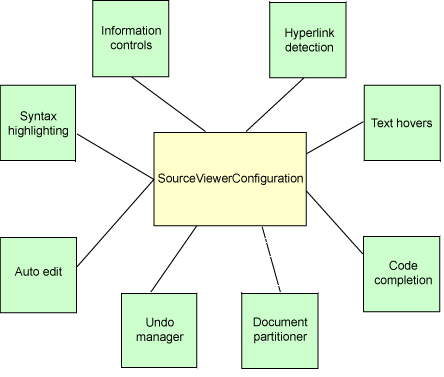
\includegraphics[width=0.5\textwidth]{figures/sourceviewerconfig}
\caption{SourceViewerConfiguration needs to setup the different functionality}
\label{fig:sourceviewerconfig}
\end{figure}

Figure \ref{fig:sourceviewerconfig} shows some of the editor functionality that needs to be configured in the \class{VdmSourceViewerConfiguration}. The configuration is changed by overriding the existing methods.


The \class{VdmDocumentProvider} bridges the file on the disk with its representation as a document in memory. We do this by extending the Eclipse class \class{FileDocumentProvider}.

\lstjava{Snippets of \java{VdmDocumentProvider}}
\begin{lstlisting}
public class VdmDocumentProvider extends FileDocumentProvider {
	...
}
\end{lstlisting}
We then override two methods:

\lstjava{Snippets of \java{VdmDocumentProvider}}
\begin{lstlisting}
@Override
protected IDocument createDocument(Object element) throws CoreException {

  IDocument document = super.createDocument(element);

  if(document instanceof IDocumentExtension3)
  {
    IDocumentExtension3 extension3 = (IDocumentExtension3) document;
    IDocumentPartitioner partitioner = 
      new VdmDocumentPartitioner(
        VdmUIPlugin.getDefault().getPartitionScanner(), 	
        VdmPartitionScanner.PARTITION_TYPES);
    extension3.setDocumentPartitioner(VdmUIPlugin.VDM_PARTITIONING, 
      partitioner);
    partitioner.connect(document);			
  }

  return document;
}
\end{lstlisting}
What we do here is creating a new document and connecting it to the partition scanner (the partition scanner is explained more in detail in the section \ref{editor:partitioning}). 




\subsection{Package editor.partitioning}
\label{editor:partitioning}
Each document is divided into one or more non-overlapping partitions. Many of the text-framework features can be configured to operate differently for each partition. Thus, an editor can have different syntax highlighting, formatting, or Content Assist for each partition \footnote{\url{http://wiki.eclipse.org/FAQ_What_is_a_document_partition\%3F}} . 




\subsection{Package editor.autoedit}

\subsection{Package editor.syntax}


